%fichier : Projet_Di4_PPGL_Astie-Teddy.tex
%Date : 03/01/2023
%Version : 1.00

\documentclass{EPUProjetDi}
\usepackage{listings}

\makeindex

%remplir les lignes suivantes avec les informations vous concernant :
\title[Projet FourmiLaby Rust]{Serveur Rust pour le projet Labyrinthe de Fourmis}

\projet{Projet de Programmation et Génie Logiciel}

\author{Teddy Astie\\ %Attention : toujours écrire d'abord le prénom puis le nom (ne pas mettre tout le nom en majuscules)
\noindent[\url{teddy.astie@etu.univ-tours.fr}]\\
}

\encadrant{Nicolas Monmarché\\ %
\noindent[\url{nicolas.monmarche@univ-tours.fr}]\\~\\
Polytech Tours\\
Département Informatique\\~ %
}

%%%%%%%%%%%%%%%%%%%%%%%%%%%%%%%%%%%%%%%%%%%%%%%%%%%%%%%%%%%%%%%%%%%%%%%%%%%%%%%%%%%%%%%%%%
\begin{document}

\maketitle

\pagenumbering{roman}
\setcounter{page}{0}

{
%on réduit momentanément l'écart entre paragraphes pour ne pas trop aérer la table des matières
\setlength{\parskip}{0em}

\tableofcontents

%\listoffigures
%rq1 : si vous n'avez pratiquement pas de figures, laissez la ligne précédente en commentaire

%\listoftables
%rq1 : si vous n'avez pratiquement pas de tables, laissez la ligne précédente en commentaire
}


\start
%%%%%%%%%%%%%%%%%%%%%%%%%%%%%%%%%%%%%%%%%%%%%%%%%%%%%%%%%%%%%%%%%%%%%%%%%%%%%%%%%%%%%%%%%%

\chapter*{Introduction}
%le 2 lignes suivantes permettent d'ajouter l'introduction à la table des matières
%et d'afficher "Introduction en haut des pages"
\addcontentsline{toc}{chapter}{\numberline{}Introduction}
\markboth{\hspace{0.5cm}Introduction}{}

Ce projet fait partie de l'ensemble des projets du "jeu de fourmis" proposé par Nicolas Monmarché. Il en constitue notamment l'un des serveurs ici le serveur codé en Rust.

\section{Rappel du principe de jeu Labyrinthe de Fourmis}

Le jeu labyrinthe de fourmis est un jeu coopératif dont l'objectif est d'obtenir le plus de points en apportant de la nourriture jusqu'au nid au travers d'un labyrinthe. Afin de faciliter les décisions des jours, un mécanisme de phéromone est mis en place, afin de déterminer le chemin pris par un joueur qui a réussi à apporter la nourriture jusqu'au nid.

L'environnement de jeu est un labyrinthe sur une grille en 2 dimensions pour lequel chaque case peut comporter éventuellement des mur dans chaque direction ainsi qu'éventuellement de la nouriture et/ou un nid. Le joueur doit trouver un chemin du nid jusqu'à une source de nourriture en évitant les murs, et si possible en prenant le plus court chemin.

Lorsque le joueur trouve de la nourriture, il émet des phéromones sur les cases qu'il traverse, jusqu'à ce qu'il arrive au nid.

Chaque joueur reçoit une copie du labyrinthe lors de son arrivée sur la partie, ainsi que régulièrement (chaque seconde) le niveau de phéromone de chaque case.

Les différentes parties intervenant dans le jeu (client et serveur) communiquent selon un protocole de communication basé sur du JSON et par du TCP/IP.

Le serveur est capable de gérer plusieurs parties en même temps, une phase de connexion/négociation est effectuée lorsque qu'un client se connecte au serveur, de plus, il est possible pour un joueur de se reconnecter à une partie après un éventuel problème de connexion.

\section{Intérêt du langage Rust dans le projet}

Initialement, les langages proposés furent le C et éventuellement le C++. Toutefois, ce projet sous-entends tout un ensemble de problèmes difficiles à gérer dans ces langages : synchronisation, gestion mémoire, ... ce qui peut être grande source de difficultés (bugs, plantages, ...) en C ou même C++\footnote{bien que les standards modernes du type C++20 aident partiellement à résoudre ces problèmes mais au prix d'un code bien plus complexe et bien en dehors du cadre de nos cours de C++}.

\begin{center}
  
\includegraphics[width=\linewidth/2]{rust-social-wide.jpg}
\end{center}

Le langage Rust qui a gagné beaucoup d'intérêt ces dernières années est décrit comme un "langage de programmation fiable, concurrent, pratique" ayant un modèle de concurrence inspiré de l'Erlang\footnote{\url{https://www.erlang.org/}} et conçu pour produire des logiciels fiables et robustes tout en garantissant une très haute performance. Ce langage a été en grande partie conçu pour éviter une grande partie des problèmes cités au dessus (synchronisation, gestion mémoire) avec des mécanismes particuliers comme par exemple système d'ownership/borrowing strict, le paramètre de durée de vie (non utilisé dans le projet), divers marqueurs, clonage non implicite, etc. De plus, le directeur technique de Microsoft Azure nous recommande d'utiliser Rust à la place de C et C++ pour des nouveaux projets\cite{markrussinovich}.

Pour toutes ces raisons et d'autres encore, le langage Rust a été choisi pour réaliser ce projet.

\chapter{Structure générale du projet}

\begin{center}
  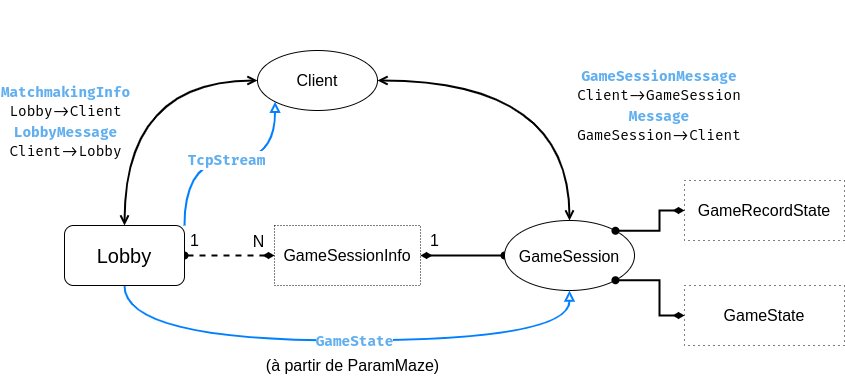
\includegraphics[width=\linewidth]{Diagramme structure.png}
  \label{fig:DiagrammeStructure}
  
  \includegraphics[width=\linewidth/2]{Légende diagramme structure.png}

  Organisation générale du projet (non exhaustif)
\end{center}

Le projet est divisé en divers composants (ou modules) intéragissants entre eux en utilisant des canaux asynchrones de type Multiple-Producer Single-Consumer disponibles dans la librairie standard Rust depuis le module \verb|syd::sync::mpsc|\footnote{\url{https://doc.rust-lang.org/std/sync/mpsc/index.html}}. Ce modèle s'apparente au modèle d'acteur\footnote{\url{https://fr.wikipedia.org/wiki/Modèle_d'acteur}} qui consiste à avoir plusieurs "acteurs" qui communiquent par passage de message, dans notre cas, hormis pour la gestion des \verb|GameSessionInfo| qui se fait par partage mémoire et comptage de référence (\verb|Arc<>| + \verb|Weak<>|), tout le reste communique par passage de message et instanciation de nouveaux acteurs.

Le projet comporte aussi d'autres parties plutôt utilitaires qui ne sont pas affichés dans le diagramme dont l'implémentation du protocole de communication (\verb|message|), l'intéraction avec la librairie de génération de labyrinthe (\verb|external::generator|) ou encore la gestion d'erreur (\verb|error|) et la structure de labyrinthe (\verb|maze|).

Le projet est relativement modulaire, et a été pensé pour être extensible (on peut par exemple ajouter des fonctionnalitées dans les modules en ajoutant de nouveaux types de message acceptés), ainsi qu'en essayant de décupler les objets en sous-objets (en particulier pour \verb|GameSession| découpé en objets plus pratiques pour implémenter certains traits (comme \verb|Serializable| pour \verb|GameState|)), ce qui peut nous permettre par exemple ici d'enregistrer l'état d'une partie dans un fichier.

\begin{center}
  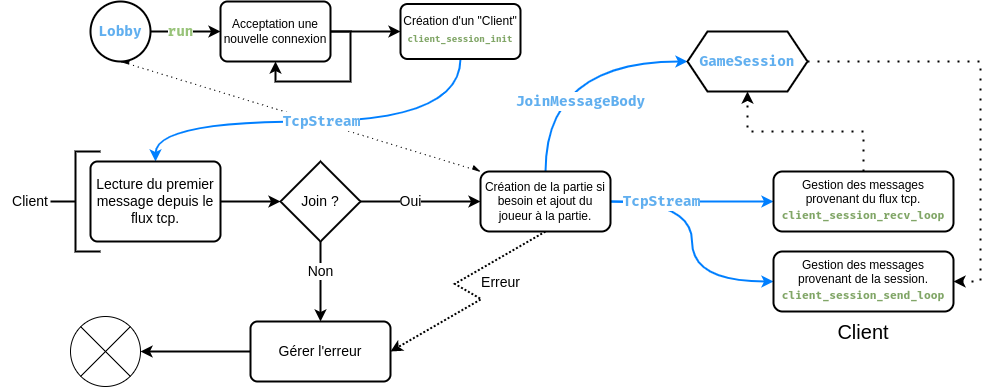
\includegraphics[width=\linewidth]{Diagramme flux.png}
  \label{fig:DiagrammeFlux}

  Flot d'exécution général
\end{center}

\chapter{Présentation des modules clés}

\section{Lobby}

L'exécution commence tout d'abord dans le \verb|Lobby| qui a deux responsabilitées.

Tout d'abord, le \verb|Lobby| accepte les différents sockets, et construit des clients.

Au même temps (dans un thread à part), le \verb|Lobby| reçoit des messages de la part des clients pour trouver une partie (\textit{matchmaking}, en créant si besoin la partie), ainsi qu'effectuer d'autres tâches de maintenance des structures de données (supprimer les références vers des parties qui n'existent plus) et gère la liste des parties en cours, des liens entre les \verb|UUID| des joueurs et leur serveur associé.

\section{Client}

Le \verb|client| est construit par le \verb|Lobby| à partir de son \verb|TcpStream|, et d'un canal vers le \verb|Lobby|. La première étape du \verb|client| est de se charger de vérifier et rediriger la négociation d'une partie avec le \verb|Lobby| afin de se connecter à une \verb|GameSession|. Une fois le client connecté à la \verb|GameSession|, ce client se charge de vérifier et rediriger tous les \verb|Message| provenant du \verb|TcpStream| jusqu'à la \verb|GameSession| ainsi que tous les messages de la \verb|GameSession| jusqu'au \verb|TcpStream|.

En cas d'erreur fatale (message inattendu, JSON invalide, erreur réseau, plantage de la parties), envoie si possible une erreur au \verb|TcpStream|, stoppe le \verb|TcpStream| puis detruit le canal du client ce qui va à terme invalider la connexion du client pour la \verb|GameSession|.

\section{GameSession}

L'acteur \verb|GameSession| pilote une \verb|GameState| à partie des messages qu'il reçoit, notamment, il gère une liste de clients connectés, gère leur éventuelle déconnection. Il gère également l'évaporation régulière des niveaux de phéromones pour chaque case ainsi l'envoi régulier des niveaux de phéromones.
De plus, il détient la \verb|GameSessionInfo|.
Une fonctionnalité expérimentale gérée par le \verb|GameSession| est l'enregistrement automatique des parties par \verb|GameRecordState|.

\section{GameState}

La structure de \verb|GameState| est l'état instantanné de la partie, il détient toutes les informations sur l'état de la partie : le labyrinthe considéré, les niveaux de phéromones, les \verb|UUID| des joueurs, et leur position ainsi que si ils détiennent de la nouriture.
Par conséquent, le \verb|GameState| n'a aucune connaissance de si un joueur concerné est actuellement connecté ou non et détient que des objets bruts ou listes, le rendant notamment compatible avec les traits \verb|Clone|, \verb|Send| et \verb|Serializable|. 

En plus de cela, cette structure implémente diverses fonction pour gérer la logique du jeu (déplacements des fourmis, actualisation des niveaux de phéromones, actualisation de l'évaporation, etc.).

\section{GameRecordState et GameRecord}

La structure de \verb|GameRecordState| définit un état d'enregistrement donc l'instant du dernier message (pour calculer les délais), les différents messages depuis le début de la partie, etc., il est utilisé pour construire à terme le \verb|GameRecord| qui est une version figée dans le marbre et \verb|Serializable| de \verb|GameRecordState|.

L'enregistrement d'une partie trace l'intégralité des messages envoyés par les joueurs, le labyrinthe considéré, ainsi que le moment auquel chaque message a été reçu, cela permet de rejouer une partie, un mécanisme expérimental pour rejouer une partie existe dans le module \verb|client::record|.

\chapter{Choix techniques et apports du Rust}

\section{Système concurrent par passage de message}

Le choix technique le plus notable dans le projet, c'est d'utiliser une approche concurrente fonctionnant principalement par passage de message à l'inverse d'une approche plutôt orientée objet à mémoire partagée.

Cette approche est particulièrement pratique pour exploiter plusieurs processeurs tout en évitant tout un ensemble de problème de synchronisation que l'on pourrait avoir avec une autre approche. De cette manière, la modélisation obtenue s'apparente au modèle d'acteur\footnote{\url{https://fr.wikipedia.org/wiki/Modèle_d'acteur}}.

L'approche orientée objet fonctionnant exclusivement par partage mémoire aurait été limitée car chercher à rendre le code parallèle aurait été ardu comme cela aurait impliqué l'utilisation d'un grand nombre de \verb|Mutex| ainsi que d'autres outils de synchronisation donc aura compliqué plusieurs parties du code. Même en négligeant le parralèlisme donc utilise un unique thread, étant donné que l'on souhaite manipuler plusieurs sockets et plusieures sessions de jeu au même moment, on aurait eu d'une manière à implémenter tout un mécanisme de gestion d'I/O asynchrone ou utiliser une librairie pour le faire à notre place, ce qui est loin d'être simple. C'est pourquoi une approche évitant le couplage est plus souhaitable.

Le Rust nous offre un large panel d'outil pour implémenter les deux approches (passage de message et mémoire partagée), ce qui est pratique car on peut suivant ce que l'on souhaite effectuer, on peut choisir une approche au lieu d'une autre. Dans notre cas, l'ensemble du projet fonctionne par passage de message à l'exception des informations des parties qui est partagée entre le \verb|Lobby| et la \verb|GameSession| (afin notamment de pouvoir déterminer si la partie concernée est en cours ou non, à l'aide de la validité de la référence que détient le \verb|Lobby| vers cette structure).

Il est utile de noter que la plupart des librairies asynchrones Rust\footnote{async-std, tokio} favorisent une approche par passage de message avec par exemple des versions adaptées de \verb|std::sync::mpsc|.

\section{Garanties de fiabilité}

Le langage Rust met en oeuvre tout un ensemble de mécanisme ayant des implications sur le code pour éviter les fuites mémoires sans pour autant nécessiter un garbage-collector (bien qu'il soit possible d'en obtenir avec des références cycliques de \verb|Rc<T>|), d'accéder à des références invalides, certains problèmes liés à l'aliasing, les \textit{race conditions}, \dots Cela peut impliquer l'utilisation de types particulier pour encapsuler nos objets si l'on veut permettre à l'objet d'être référencé à plusieurs endroits (\verb|Rc<T>| et \verb|Arc<T>| similaires à \verb|std::shared_ptr| en C++) ou encore si l'objet peut être modifié par plusieurs thread (\verb|Mutex<T>|), etc\dots

Cela prend notamment la forme de \textit{traits} ($\approx$ interface) spécifiques indiquant si l'objet peut être transféré dans un autre thread ou encore partagée entre plusieurs threads\footnote{\url{https://doc.rust-lang.org/nomicon/send-and-sync.html}}.

De cette manière, un grand nombre d'éventuels problèmes de synchronisation ou de gestion mémoire sont évités ou simplifiés. Toutefois, ce fonctionnement est assez unique et pas très habituel dans d'autres langages de programmation, ce qui peut rendre compliqué l'apprentissage du Rust aux développeurs qui ne sont pas habitués à ces concepts.

\section{Traitement des messages à l'aide des \textit{tagged union} et du \textit{pattern matching}}

L'une des fonctionnalitées du langage Rust les plus pratiques pour implémenter le traitement des messages du protocole utilisé dans le jeu mais aussi ceux pour le passage de message est le pattern matching couplé aux \textit{tagged unions}\footnote{\url{https://en.wikipedia.org/wiki/Tagged_union}}\footnote{\url{https://doc.rust-lang.org/book/ch06-00-enums.html}}. Cet outil nous permet de créer des \textit{types somme} qui est une sorte d'énumération (plus précisément, une version améliorée des énumérations), mais dont chaque variant peut avoir des valeurs ou non (sous la forme d'une valeur, tuple, structure, ...). On peut par exemple définir un union taggué pouvant recevoir chaque type de message supporté par le protocole ainsi que leurs valeurs.

Cette fonctionnalité est également très utilisée dans les fonctionnalitées de base du langage, nottament \verb|Option<T>|\footnote{\url{https://doc.rust-lang.org/core/option/index.html}}, \verb|Result<T, E>|\footnote{\url{https://doc.rust-lang.org/core/result/index.html}}(gestion d'erreur), et bien d'autres.

\begin{center}
  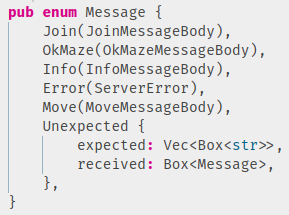
\includegraphics[width=\linewidth/3]{EnumMessage.png}
  \label{fig:EnumMessage}

  Enumeration pour les messages du protocole de communication
\end{center}

En utilisant \verb|match|, il est possible de prendre une décision pour chaque variant de l'union taggué/enumération, tout en destructurant chaque variant, ce qui permet de facilement utiliser ces objets. Il est également possible de faire du "pattern matching" à l'aide de match y compris sur l'élément à l'intérieur du match.

\begin{center}
  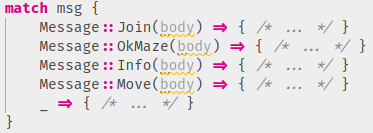
\includegraphics[width=\linewidth/2]{MatchMessage.png}
  \label{fig:MatchMessage}

  Utilisation de match sur un message suivant son type
\end{center}

Cette fonctionnalité est extensivement utilisée pour le traitement de message, que ce soit provenant d'un client distant (socket), ou pour le passage de messages entre les acteurs. Il existe une alternative dans le cas où un seul cas particulier nous intéresse (\verb|if let|\footnote{\url{https://doc.rust-lang.org/book/ch06-03-if-let.html}})

\section{Sérialisation de données à l'aide de serde et serde-json}

Serde\footnote{\url{https://serde.rs/}} est un framework de sérialisation de donnéees Rust (ce framework fait parties de \url{https://blessed.rs}), il permet de rendre des types \verb|Serialize| et \verb|Deserialize| de manière automatiques (en utilisant \verb|derive|) ou non ainsi que personaliser la manière dont est structuré la donnée. En complément à cette librairie est peut être implémenté une librairie pour sérialiser et désérialiser différents format de sérialisation, en particulier pour notre projet le format JSON à l'aide de \verb|serde-json|\footnote{\url{https://crates.io/crates/serde_json}}.

De cette manière, en utilisant , on peut très facilement sérialiser ainsi que désérialiser l'ensemble des messages que peut envoyer ou recevoir le serveur, ce qui s'avère extrêmement pratique pour implémenter le protocole.

De plus, cela permet de facilement changer le format de sérialisation si nécessaire sans impliquer de grands changements dans le reste code.

%--------------------------------------------------------------------------------
\chapter*{Conclusion}
\addcontentsline{toc}{chapter}{\numberline{}Conclusion}
\markboth{Conclusion}{}

\label{sec:conclusion}

%--------------------------------------------------------------------------------
%exemple de bibliographie
\begin{thebibliography}{99}
\label{sec:biblio}
\bibitem{markrussinovich}  \url{https://www.zdnet.com/article/programming-languages-its-time-to-stop-using-c-and-c-for-new-projects-says-microsoft-azure-cto/}
\bibitem{ref2}  détail bibliographique de la ref2
\bibitem{ref3}  détail bibliographique de la ref3
\bibitem{ref4}  détail bibliographique de la ref4
\bibitem{ref5}  détail bibliographique de la ref5
\end{thebibliography}


%--------------------------------------------------------------------------------
%si on donne des annexes :
\appendix
\addcontentsline{toc}{part}{\numberline{}Annexes}

%--------------------------------------------------------------------------------

\chapter{Liens utiles\label{sec:liens_utiles}}
Voici une petite liste d'url intéressantes au sujet de ce projet :

\begin{itemize}
\item Gitlab du projet \url{https://scm.univ-tours.fr/21906867t/serveur-fourmi}
\item Site officiel du Rust \url{https://www.rust-lang.org/fr/}
\item Référentiel de documentation Rust \url{https://www.rust-lang.org/fr/learn}
\item Référence en magie noire en Rust \url{https://doc.rust-lang.org/nomicon/}
\item Documentation de serde \url{https://serde.rs}
\end{itemize}




%--------------------------------------------------------------------------------
%index : attention, le fichier dindex .ind doit avoir le même nom que le fichier .tex
%\printindex

%--------------------------------------------------------------------------------
%page du dos de couverture :

\resume{Le méta-projet de jeu de fourmis est un jeu de simulation de fourmis multijoueur utilisant une architecture Client-Serveur. Ce projet propose une implémentation du serveur dans le langage Rust, et permet ainsi de mesurer l'intérêt de ce langage pour ce projet. Il fait partie avec le projet C++ des 2 implémentations du serveur pour ce jeu. }

\motcles{Rust, Simulation, Fourmis, Programmation Concurrente, Programmation Fonctionelle, Multithreading, Réseau, Sérialisation, Jeu, TCP}

\abstract{The meta-project of "ant simulation game" is a multiplayer ant simulation serious-game based on a Client-Server architecture. This project offer a Rust implementation for the server, and highlights the benefits of this programming language in this project. It is along with the C++ project one of the implementations of the server for this game.}

\keywords{Rust, Simulation, Ant, Concurrent Programming, Functionnal Programming, Multithreading, Network, Serialization, Game, TCP}

\makedernierepage


\end{document}
%%FIN du fichier